%%%%%%%%%%%%%%%%%%%%%%%%%%%%%%%%%%%%%%%%%
% Programming/Coding Assignment
% LaTeX Template
%
% This template has been downloaded from:
% http://www.latextemplates.com
%
% Original author:
% Ted Pavlic (http://www.tedpavlic.com)
%
% Note:
% The \lipsum[#] commands throughout this template generate dummy text
% to fill the template out. These commands should all be removed when 
% writing assignment content.
%
% This template uses a Perl script as an example snippet of code, most other
% languages are also usable. Configure them in the "CODE INCLUSION 
% CONFIGURATION" section.
%
%%%%%%%%%%%%%%%%%%%%%%%%%%%%%%%%%%%%%%%%%

%----------------------------------------------------------------------------------------
%	PACKAGES AND OTHER DOCUMENT CONFIGURATIONS
%----------------------------------------------------------------------------------------

\documentclass[a4paper]{article}

\usepackage{fancyhdr} % Required for custom headers
\usepackage{lastpage} % Required to determine the last page for the footer
\usepackage{extramarks} % Required for headers and footers
\usepackage[usenames,dvipsnames]{color} % Required for custom colors
\usepackage{graphicx} % Required to insert images
\usepackage{listings} % Required for insertion of code
\renewcommand*{\lstlistingname}{代码} % change "Listing <ref> to 代码 <ref>
\usepackage{courier} % Required for the courier font
\usepackage{lipsum} % Used for inserting dummy 'Lorem ipsum' text into the template

\usepackage[UTF8]{ctex} % Required for Chinese character
\usepackage{tocloft} % Required for beautiful toc
\usepackage[hidelinks]{hyperref} % Required for clickable toc
\hypersetup{
    colorlinks,
    citecolor=black,
    filecolor=black,
    linkcolor=black,
    urlcolor=black
}
\usepackage[title]{appendix} % Required for appendix
\usepackage{float}
\usepackage{amsmath} % used for \text{} in math formula


% used for beautiful table
\usepackage{booktabs} 
\usepackage[T1]{fontenc}
\usepackage{tabu}
\usepackage{longtable}
\usepackage[table]{xcolor}


% Margins
\topmargin=-0.45in
\evensidemargin=0in
\oddsidemargin=0in
\textwidth=6.5in
\textheight=9.0in
\headsep=0.25in

\linespread{1.1} % Line spacing

% Set up the header and footer
\pagestyle{fancy}
\lhead{\hmwkAuthorName} % Top left header
\chead{\hmwkClass\ (\hmwkClassInstructor\ \hmwkClassTime): \hmwkTitle} % Top center head
\rhead{\firstxmark} % Top right header
\lfoot{\lastxmark} % Bottom left footer
\cfoot{} % Bottom center footer
\rfoot{Page\ \thepage\ of\ \protect\pageref{LastPage}} % Bottom right footer
\renewcommand\headrulewidth{0.4pt} % Size of the header rule
\renewcommand\footrulewidth{0.4pt} % Size of the footer rule

\setlength\parindent{0pt} % Removes all indentation from paragraphs

%----------------------------------------------------------------------------------------
%	CODE INCLUSION CONFIGURATION
%----------------------------------------------------------------------------------------

\definecolor{MyDarkGreen}{rgb}{0.0,0.4,0.0} % This is the color used for comments
\lstloadlanguages{c} % Load Perl syntax for listings, for a list of other languages supported see: ftp://ftp.tex.ac.uk/tex-archive/macros/latex/contrib/listings/listings.pdf
\lstset{language=c, % Use Perl in this example
        frame=single, % Single frame around code
        basicstyle=\small\ttfamily, % Use small true type font
        keywordstyle=[1]\color{Blue}\bf, % Perl functions bold and blue
        keywordstyle=[2]\color{Purple}, % Perl function arguments purple
        keywordstyle=[3]\color{Blue}\underbar, % Custom functions underlined and blue
        identifierstyle=, % Nothing special about identifiers                                         
        commentstyle=\usefont{T1}{pcr}{m}{sl}\color{MyDarkGreen}\small, % Comments small dark green courier font
        stringstyle=\color{Purple}, % Strings are purple
        showstringspaces=false, % Don't put marks in string spaces
        tabsize=4, % 5 spaces per tab
        %
        % Put standard Perl functions not included in the default language here
        % morekeywords={rand},
        morekeywords = [1]{uint16_t, uint32_t, uint8_t, int16_t, int8_t, int32_t}
        %
        % Put Perl function parameters here
        morekeywords=[2]{on, off, interp, __attribute__},
        %
        % Put user defined functions here
        morekeywords=[3]{test},
       	%
        morecomment=[l][\color{Blue}]{...}, % Line continuation (...) like blue comment
        numbers=left, % Line numbers on left
        firstnumber=1, % Line numbers start with line 1
        numberstyle=\tiny\color{Blue}, % Line numbers are blue and small
        stepnumber=2, % Line numbers go in steps of 5,
        firstnumber=1
}

% define C style
\definecolor{main-color}{rgb}{0.6627, 0.7176, 0.7764}
\definecolor{back-color}{rgb}{0.1686, 0.1686, 0.1686}
\definecolor{string-color}{rgb}{0.3333, 0.5254, 0.345}
\definecolor{key-color}{rgb}{0.8, 0.47, 0.196}
\lstdefinestyle{mystyle}
{
    language = C++,
    basicstyle = {\small\ttfamily},
    stringstyle = {\color{Mahogany}},
    keywordstyle = {\color{blue}},
    keywordstyle = [2]{\color{Mahogany}},
    keywordstyle = [3]{\color{blue}},
    keywordstyle = [4]{\color{blue}},
    otherkeywords = {__attribute__,<<,>>,++},
    morekeywords = [2]{__attribute__},
    morekeywords = [3]{<<, >>},
    morekeywords = [4]{++, uint16_t, uint32_t, uint8_t, \#define},
}


% Creates a new command to include a perl script, the first parameter is the filename of the script (without .pl), the second parameter is the caption

\newcommand{\shfilescript}[3]{
\begin{itemize}
\item[]\lstinputlisting[caption=#2, label=lst:#1, language=sh]{#3}
\end{itemize}
}
\newcommand{\shscript}[3]{
\begin{itemize}
\item[]\begin{lstlisting}[label=lst:#1, caption=#2] #3 \end{lstlisting}
\end{itemize}
}

%----------------------------------------------------------------------------------------
%	DOCUMENT STRUCTURE COMMANDS
%	Skip this unless you know what you're doing
%----------------------------------------------------------------------------------------

% Header and footer for when a page split occurs within a problem environment
\newcommand{\enterProblemHeader}[1]{
\nobreak\extramarks{#1}{#1 见下页\ldots}\nobreak{} 
\nobreak\extramarks{接上页}{#1 见下页\ldots}\nobreak{}
}

% Header and footer for when a page split occurs between problem environments
\newcommand{\exitProblemHeader}[1]{
\nobreak\extramarks{接上页}{#1 见下页\ldots}\nobreak{}
\nobreak\extramarks{#1}{}\nobreak{}
}
% TODO:code here enable the number before section, but it disable the numbering of problems
%\setcounter{secnumdepth}{0} % Removes default section numbers
\newcounter{homeworkProblemCounter} % Creates a counter to keep track of the number of problems

\newcommand{\homeworkProblemName}{}

\newenvironment{homeworkProblem}[1][Problem \arabic{homeworkProblemCounter}]{ % Makes a new environment called homeworkProblem which takes 1 argument (custom name) but the default is "Problem #"
\stepcounter{homeworkProblemCounter} % Increase counter for number of problems
\renewcommand{\homeworkProblemName}{#1} % Assign \homeworkProblemName the name of the problem
\section{\homeworkProblemName} % Make a section in the document with the custom problem count
\enterProblemHeader{\homeworkProblemName} % Header and footer within the environment
}{
\exitProblemHeader{\homeworkProblemName} % Header and footer after the environment
}

\newcommand{\problemAnswer}[1]{ % Defines the problem answer command with the content as the only argument
\noindent\framebox[\columnwidth][c]{\begin{minipage}{0.98\columnwidth}#1\end{minipage}} % Makes the box around the problem answer and puts the content inside
}

\newcommand{\homeworkSectionName}{}
\newenvironment{homeworkSection}[1]{ % New environment for sections within homework problems, takes 1 argument - the name of the section
\renewcommand{\homeworkSectionName}{#1} % Assign \homeworkSectionName to the name of the section from the environment argument
\subsection{\homeworkSectionName} % Make a subsection with the custom name of the subsection
\enterProblemHeader{\homeworkProblemName\ [\homeworkSectionName]} % Header and footer within the environment
}{
\enterProblemHeader{\homeworkProblemName} % Header and footer after the environment
}


\newcommand{\codev}[1]{\textsf{#1}}
%----------------------------------------------------------------------------------------
%	NAME AND CLASS SECTION
%----------------------------------------------------------------------------------------

% table color
\definecolor{tableHeader}{RGB}{245, 245, 245}
\definecolor{tableLineOne}{RGB}{245, 245, 245}
\definecolor{tableLineTwo}{RGB}{224, 224, 224}
\newcommand{\tableHeaderStyle}{
    \rowfont{\leavevmode\color{white}\bfseries}
    \rowcolor{tableHeader}
}

%----------------------------------------------------------------------------------------

\newcommand{\hmwkTitle}{操作系统原理实验\ \#7(保护模式)} % Assignment title
\newcommand{\hmwkDueDate}{Wednesday,\ June\ 13,\ 2018} % Due date
\newcommand{\hmwkClass}{16级计科\ 7班} % Course/class
\newcommand{\hmwkClassTime}{周一9-10节} % Class/lecture time
\newcommand{\hmwkClassInstructor}{凌应标} % Teacher/lecturer
\newcommand{\hmwkAuthorName}{颜彬} % Your name
\newcommand{\hmwkAuthorId}{16337269} % Your id 

%----------------------------------------------------------------------------------------
%	TITLE PAGE
%----------------------------------------------------------------------------------------

\usepackage{titling}

\title{
\vspace{2in}
\textmd{\textbf{\hmwkClass:\ \hmwkTitle}}\\
\normalsize\vspace{0.1in}\small{Due\ on\ \hmwkDueDate}\\
\vspace{0.1in}\large{\textit{\hmwkClassInstructor\ \hmwkClassTime}}
\vspace{3in}
}

\author{\textbf{\LARGE{\hmwkAuthorName}} \\ \\ \textbf{\LARGE{\hmwkAuthorId}}}
\date{} % Insert date here if you want it to appear below your name
%----------------------------------------------------------------------------------------

\begin{document}
% \begin{titlingpage} % This is for ignore page number in first page. package titling

\maketitle

%----------------------------------------------------------------------------------------
%	TABLE OF CONTENTS
%----------------------------------------------------------------------------------------

% \setcounter{tocdepth}{2} % Uncomment this line if you don't want subsections listed in the ToC
% set depth in toc

% \renewcommand{\cftsecleader}{\cftdotfill{\cftdotsep}} % used for dots between <section> and <page>

\renewcommand{\contentsname}{Content} % force the word to be "content
\newpage
\tableofcontents
\addtocontents{toc}{~\hfill\textbf{Page}\par}
\newpage

% below are document body


% To have just one problem per page, simply put a \clearpage after each problem
\section{实验目的}
在实验六或更后的原型基础上,进化你的原型操作系统,原型保留原有特征的
基础上,设计满足下列要求的新原型操作系统:\\ 

实现控制的基本原语 do_fork() 、 do_wait() 、 do_exit() 、 blocked() 和 wakeup()\\ 

内核实现三系统调用 fork() 、 wait() 和 exit() ,并在 c 库中封装相关的系统调用\\ 

编写一个 c 语言程序,实现多进程合作的应用程序\\ 
\section{实验过程}
    \subsection{fork逻辑}
    \begin{figure}
    \begin{itemize}
    \item[] \begin{lstlisting}[language=C, label=lst:fork, caption=C库中封装的fork]
#define fork() \
({\
    cli();\
    int32_t __fork_ret;\
    __asm__(\
        "movl $0x02, %%eax\n"\
        "int $0x80\n"\
        : "=r"(__fork_ret)\
        :\
    );\
    sti();\
    __fork_ret;\
})
    \end{lstlisting}
    \end{itemize}
    \end{figure}
    如代码\ref{lst:fork}所示,将fork封装到C函数库中。在进入fork的前后要关中断和开中断。\\ 

    本代码最重要的细节在于,它不以函数的形式实现。这是因为函数结束时的语句一般是leave和ret。这两条
    语句会对esp的值有影响。但是在fork完后,子进程会继承父进程的eip(在本项目的实现中,是这样处理的)。
    所以子进程被调度后,会继续执行fork函数的后半部分。为了避免fork的leave 和ret弄乱子进程的esp和
    ebp,fork不应实现成函数调用。\\ 

    另一种实现的方法是,修改子进程的eip,使得子进程被调度时,返回到fork的下一条语句中。 \\ 

    由于fork有返回值,故这里利用了C语言的$({...})$语法。这个语法中,C程序会把...中的代码全部执行完,
    然后把...中的最后一个表达式作为整个表达式的值。这样,在程序调用int pid = fork();时,可以恰好
    把pid赋为fork的返回值。
    \subsection{sys_fork逻辑}
    在fork中,通过调用0x80中断的0x2号功能实现fork。
    \begin{figure}
    \begin{itemize}
    \item[] \begin{lstlisting}[language=C, label=lst:sys_fork, caption=sys_fork逻辑]
fn_ptr sys_call_table[] = {
    test_print, print_hello, sys_fork, sys_wait, sys_exit
};

...

int sys_fork() {
    printks("[debug]fork\n");
    int32_t pindex = first_empty_pcb();
    if (pindex == -1) {
        return -1;
    }
    copy_process(pindex, current);
    return PCB_List[current].register_image.eax;
}

    \end{lstlisting}
    \end{itemize}
    \end{figure}
    如代码\ref{lst:sys_fork}所示。\\ 

    sys_call_table是一个函数数组,存储着若干函数的首地址。在调用0x80号中断时,
    功能号会成为索引,跳转到该地址表中。所以fork的0x2功能号会跳转到函数sys_fork.
    其中数组类型fn_ptr是一个typedef,类型是int (*) (),即返回int的,不接受参数的
    函数。\\ 

    在sys_fork中,首先调用first_empty_pcb得到第一个空闲的pcb表。然后调用copy_process
    ,将当前的pcb表复制到空闲的pcb表中。随后显式地返回当前进程的eax的值。

    \subsection{copy_process逻辑}
    \begin{figure}
    \begin{itemize}
    \item[] \begin{lstlisting}[language=C, label=lst:copy_process, caption=copy_process的主要代码]
void copy_process(int32_t dst_index, int32_t src_index) {
    struct RegisterImage* dst = &PCB_List[dst_index].register_image;
    struct RegisterImage* src = &PCB_List[src_index].register_image; 
    int32_t new_pid = last_pid++;

    src->eax = new_pid;
    dst->eax = 1;
    dst->ecx = src->ecx;
    ...
    dst->cs = src->cs;

    int32_t esp_offset = ProcessStack(src_index) - src->esp;
    int32_t ebp_offset = ProcessStack(src_index) - src->ebp;
    _rev_memcpy((void*)ProcessStack(dst_index), (void*)ProcessStack(src_index), 1024);
    dst->esp = ProcessStack(dst_index) - esp_offset;
    dst->ebp = ProcessStack(dst_index) - ebp_offset;

    uint32_t* pesp = (uint32_t*)dst->esp;
    *(pesp + OFFSET_EAX) = dst->eax;
    ...
    *(pesp + OFFSET_EAX) = dst->eax;

    PCB_List[dst_index].state = TASK_INTERRUPTIBLE;
    PCB_List[dst_index].pid = new_pid;
    PCB_List[dst_index].parent_id = src_index;
}
    \end{lstlisting}
    \end{itemize}
    \end{figure}
    如代码\ref{lst:copy_process}所示。\\ 

    首先将源PCB中的寄存器副本复制到目的PCB中。源和目的的eax需要根据fork的语义
    特殊处理。\\ 

    目的esp和ebp需要特殊地计算。程序为每个(内核)进程分配固定的栈空间。所以PCB
    索引和栈空间可以相互计算的。在fork后,旧esp和ebp相对于旧栈的位置,等于新
    esp和新ebp相对于新栈的位置。利用这个条件,可以求出新esp和新ebp。\\ 

    由于实验6中,进程切换的寄存器都是通过在栈中Pop来恢复的(实现细节问题),故
    此处需要把部分寄存器中PCB中手动复制到栈中,覆盖掉旧的内容。这是通过计算栈中
    寄存器(如eax)和栈顶的相对位置来实现的。\\ 

    最后,设置pid, parent_pid,以及进程的状态。
    \subsection{_rev_memcpy的实现}
    _rev_memcpy是反向内存复制的函数。它专门用来在fork中复制栈的值。\\ 

    由于栈从高地址增长到低地址,采用反向内存复制会更便于编程。该函数暂不考虑跨段
    的问题。
\section{实验结果}
    \subsection{fork测试}
    \begin{figure}[!hbt]
    \begin{itemize}
    \item[] \begin{lstlisting}[language=C, label=lst:testcase, caption=测试样例代码]
int main(){    
    sti();
    int id = fork();
    if (id == 1) {
        printks("111\n");
        int id2 = fork();
        if (id2 == 1) {
            printks("333\n");
        } else {
            printks("444\n");
        }
    } else {
        printks("222\n");
        int id2 = fork();
        if (id2 == 1) {
            printks("555\n");
        } else {
            printks("666\n");
        }
    }
    while(1);
    return;
}
void second_process() {
    int id = fork();
    if (id == 1) {
        printks("777\n");
    } else {
        printks("888\n");
    }
    while(1);
}
    \end{lstlisting}
    \end{itemize}
    \end{figure}
    测试样例的代码如\ref{lst:testcase}所示。\\ 
    
    在主进程中,通过fork产生进程2和3.在进程2和3中,分别再调用fork,产生进程4和5.
    通过在各个分支中输出111到666,可以检验fork的确正确工作了。\\ 

    程序初始化时,会利用实验6的成果,手动产生新进程。在新进程中,同样调用fork,
    并输出777和888。当在屏幕上最终显示111到888,且恰好显示一次时,说明所有的
    fork都正常工作。\\ 

    fork正常工作的情景如图\ref{fig:ts_n_fork}所示。
    \begin{figure}
        \begin{center}
        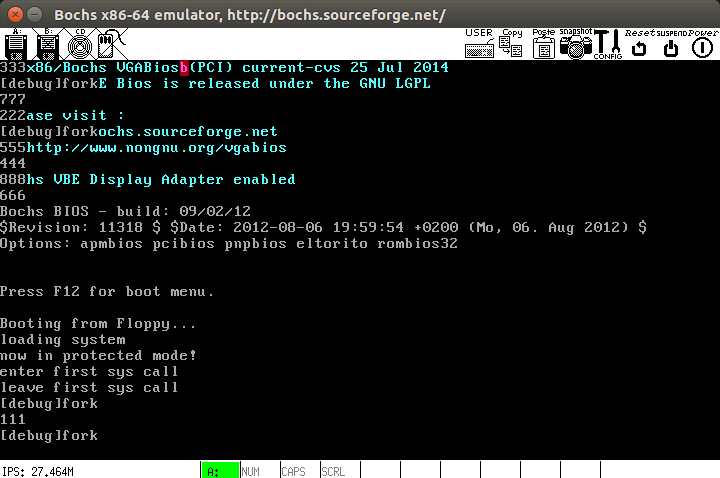
\includegraphics[scale=0.8]{./assets/pm-ex7-taskswitch-and-fork.png}
        \caption{进程切换和fork结合的测试样例\label{fig:ts_n_fork}} 
        \end{center} 
    \end{figure} 
    \subsection{wait和exit测试}
    在输出888的分支之前加入wait指令,888将不会输出,如图\ref{fig:wait}所示。\\

    但是在777的分支中加入exit指令后,由于子进程的exit解除了父进程的
    阻塞,888分支又可以再次输出到屏幕上。如图\ref{fig:exit}所示。\\ 

    值得注意的是,wait + exit的情况和一开始的图\ref{fig:ts_n_fork}不同。
    区别在于,各个进程被调度的顺序是不同的。\\
    
    \begin{figure}
    \begin{minipage}{0.48\textwidth}
        \centering
        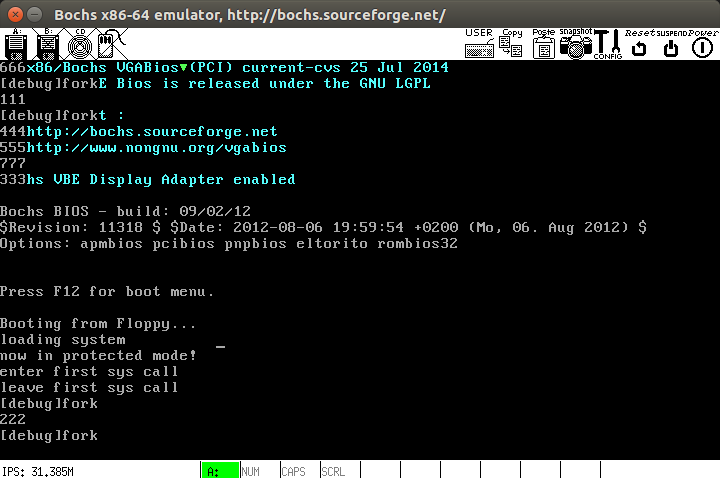
\includegraphics[width=\linewidth]{assets/pm-ex7-wait.png}
    \caption{加入一条wait指令的图片} \label{fig:wait}
    \end{minipage}\hfill
    \begin{minipage}{0.48\textwidth}
        \centering
        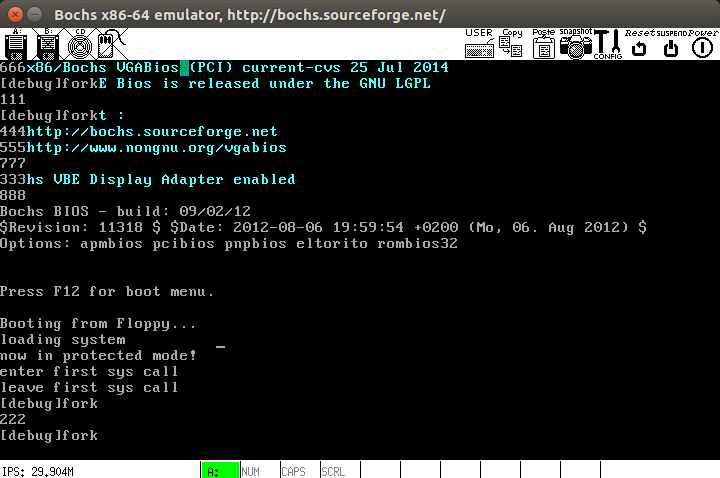
\includegraphics[width=\linewidth]{assets/pm-ex7-wait-and-exit.png}
    \caption{再加入exit指令后的图片} \label{fig:exit}
    \end{minipage}
    \end{figure}    
\section{实验总结}
    \subsection{实验心得}
    实验七拖得比较晚才交,因为我尝试了保护模式,在保护模式下重做了前面的
    几个实验,并最终实现了实验7.保护模式耗费了我不少时间。其中无数的
    试错和重写,让我的代码改了又改。\\ 

    这个实验我感觉略有困难,难度不亚于实验6。这是因为我之前参考了Linux
    的保护模式的实现,其在中断方面和进程切换方面,思路和课内的思路(也是
    大部分同学的思路)都不一样。这导致了我在做实验7时,几乎把进程切换和
    系统调用又再重写了一遍。其中还陷入许多常规保护错误中。debug比较困难。\\ 

    遇到最坑的一点是,汇编代码中的label,在C程序中,需要用&label的方式
    取得它的地址。我在做栈切换时,需要取得汇编中栈的起始地址,但一直不知道
    要加&号,导致取出来的值非常奇怪(实际上取出来的是label标签处内存的值)。\\ 

    在fork中把栈复制后,需要把新进程的esp和ebp正确地设置,由于历史实现
    的问题,进程在恢复时,除了ss和sp以外的所有寄存器的值都是从栈中恢复的。
    所以copy_process还要负责把栈中的某个位置的寄存器的值正确地修改。
    \subsection{BUG汇总}\label{sec:bug}
\begin{appendices}
\section{参考文献} \label{sec:reference}
\begin{enumerate}
    \item https://blog.csdn.net/longintchar/article/details/50602851 \\
    16位和32位汇编指令的不同(尤其是push指令)
    \item https://www.ibiblio.org/gferg/ldp/GCC-Inline-Assembly-HOWTO.html\#s1 \\
    GCC 内嵌汇编的书写。
  \end{enumerate}
\end{appendices}
\end{document}
